\documentclass[a4paper]{article}
\usepackage[polish]{babel}
\usepackage[utf8]{inputenc}
\usepackage{polski}
\usepackage[T1]{fontenc}
\frenchspacing
\usepackage{indentfirst}
\usepackage{graphicx} % Required for inserting images
\graphicspath{{./pictures/}}
\title{Zadania-Jan Rolka}
\author{Jan Rolka}
\date{Październik 2023}

\begin{document}
\section{Jan Rolka}
\label{sec:Jan Rolka}

\subsection{Przykładowe wyrażenie matematyczne}

$$
\sum_{k=1}^{\infty}\frac{1}{k^2} = \frac{\pi^2}_{6}   
$$ \\

Tutaj akurat mój ukochany problem bazylejski
\\\\

\subsection{Przykładowe zdjęcie}


\includegraphics[scale=0.25]{pictures/ObrazkiJR/Trollface}\\

Jeżeli urazilem to przepraszam

\subsection{}section{Przykładowe listy}

\begin{enumerate}
    \item koty
    \item psy
    \item myszy
    \item świnki morskie
\end{enumerate}
\\\\
\begin{itemize}
    \item jabłka
    \item gruszki
    \item śliwki
    \item banany
\end{itemize}

\begin{center}

\subsection{Formatowanie na przykładzie inwokacji Mickiewicza}

\underline{Litwo! Ojczyzno moja! ty jesteś jak zdrowie.} \emph{Ile cię trzeba cenić, ten tylko się dowie, Kto cię stracił.} \textbf{Dziś piękność twą w całej ozdobie.}\Huge{Widzę i opisuję, bo tęsknię po tobie.}

\end{center}

\begin{figure}
    \centering
    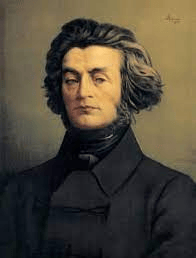
\includegraphics[scale=0.5]{pictures/ObrazkiJR/Mickiewicz}
    \caption{Adam Mickiewicz}
    \label{fig:Mickiewicz}
\end{figure}

~\ref{tab:TabelaJanRolka} 
\begin{table}
\begin{center}
\caption{Największe miasta Polski pod względem liczby ludności}
\begin{tabular}{|1||l|l|}
\hline Miasto & Ludność & Powierzchnia (w km^2) \\ \hline \hline
Warszawa & 1765000 &  517,2\\
Kraków & 804000 & 326,85 \\
Wrocław & 674000 & 296 \\ \hline
\end{tabular}
\end{center}
\end{table}


\end{document}